\documentclass{report}

\usepackage[utf8]{inputenc} % Charakter-Kodierung
\usepackage[german]{babel} % Sprache

\usepackage[table,xcdraw]{xcolor} % Tabellen Farben
\usepackage{tabularx} % Dynamische Tabellenbreite
\usepackage{tcolorbox} % Graue Boxen
\usepackage{hyperref} % url Umgebung
\usepackage{todonotes} % Notizen
\usepackage{natbib} % Bibliographie
\usepackage{fancyhdr} % Header und Footer
\usepackage{multirow} % Multizeile
\usepackage{geometry} % Page layout
\usepackage{color} % Text Farben
\usepackage[section]{placeins}%Stops pictures from moving around EVERYWHERE

% Page layout
\geometry{
	bottom=3.5cm,
	headheight=180pt
}

% Nummerierung der ersten Seiten verhindern
\pagenumbering{gobble}

% Bibstyle
\bibliographystyle{plain}

% Header / Footer
\fancypagestyle{plain}{
	\fancyhf{}% Clear header/footer
	\fancyhead[R]{\includegraphics[width=4cm]{img/cau-logo-2017}} % Rechter header
	\fancyhead[L]{\leftmark} % Linker header
	\fancyfoot[R]{\thepage} % Rechter footer
	\fancyfoot[L]{
\includegraphics[width=1cm]{img/se-logo}} % Linker footer
}
\pagestyle{plain}

\renewcommand{\headrulewidth}{0.5pt} % Unnötige Informationen der Kapitelangabe
\renewcommand{\footrulewidth}{0.2pt} % entfernen
\renewcommand{\chaptermark}[1]{\markboth{{#1}}{}}




% Zahlen für Fußnoten
\renewcommand{\thefootnote}{\arabic{footnote}}
\renewcommand{\thempfootnote}{\arabic{mpfootnote}}

%%%%% Ausfüllen %%%%%

% Gruppenname
\newcommand{\gruppenname}{Gruppe WSP31}

% Projektname
\newcommand{\projektname}{SWARM Composer }

% Semester
\newcommand{\semester}{SoSe18}


% Titelseite

\title{
	\vspace*{-3cm}
	Pflichtenheft\\
	\projektname\\
	-\\
	\color{gray}
	Softwareprojekt \semester\\
	\gruppenname\\
	\vspace*{5mm}
	
\includegraphics[width=\textwidth]{img/Logo}
}

\author{
	\begin{tabular}{r l@{\hspace{8\tabcolsep}} r}
		Lorenz & Boguhn & \multirow{8}{*}{ 
\includegraphics{img/se-logo} } \\
		Lennart & Brandt \\
		Arved & Hansen \\
		Matthias & Johannsen \\
		Lars & Jürgensen \\
		Birger & Thormählen \\
		Björn & Vonheiden\\
		Thomas & Zacher \\
	\end{tabular}
}

\date{\today}





% Dokument

\begin{document}
	\maketitle

	\tableofcontents

	\chapter{Lizenz}\label{chp:lizenz}
	\pagenumbering{arabic} % Nummerierung starten
	
Copyright 2018 \projektname\\
\\
Licensed under the Apache License, Version 2.0 (the ``License'');
you may not use this file except in compliance with the License.
You may obtain a copy of the License at
\begin{center}
 	http://www.apache.org/licenses/LICENSE-2.0
\end{center}
Unless required by applicable law or agreed to in writing, software
distributed under the License is distributed on an ``AS IS'' BASIS,
WITHOUT WARRANTIES OR CONDITIONS OF ANY KIND, either express or implied.
See the License for the specific language governing permissions and
limitations under the License.


	\chapter{Zielbestimmungen}\label{chp:zielbestimmungen}
	\section{Musskriterien}
\subsection{Webseite und App}
\begin{itemize}
\item Beide zeigen die Kompatibilität einer Kombination von Diensten an.
\item Man kann sich in den Account einloggen.
\item Man kann gespeicherte Kombinationen suchen, auswählen und ansehen.
\item Man kann Dienste über ihren Namen und ihre Tags suchen.
\end{itemize}

\subsection{Webseite}
\begin{itemize}
\item Administratoren können Dienste und Formate hinzufügen
\item Administratoren können Dienste bearbeiten und updaten, bei Formatänderungen muss ein neuer Dienst erstellt werden.
\item Administratoren können andere Nutzer zum Administrator ernennen.
\item Man kann einen Account mit Name, Vorname, Titel, Organisation, E-Mail Adresse und Passwort erstellen.
\item Eingeloggte Benutzer können Kombinationen erstellen, speichern und freigeben.
\item Die Freigabe für Kombinationen wird für einzelne Personen oder auf öffentlich gesetzt.
\end{itemize}

\subsection{App}
\begin{itemize}
\item Man kann Kombinationen per E-Mail versenden.
\end{itemize}

\section{Sollkriterien}
\subsection{Webseite}
\begin{itemize}
\item Man kann Gruppen erstellen und Kombinationen für diese freigeben.
\end{itemize}

\section{Kannkriterien}
\subsection{Webseite}
\begin{itemize}
\item Man kann sich Kopien der Kombinationen erstellen und diese dann verändern.
\item Man kann Kombinationen per E-Mail versenden.
\end{itemize}

\subsection{App}
\begin{itemize}
\item Administratoren können Dienste und Formate hinzufügen
\item Administratoren können Dienste bearbeiten und updaten, bei Formatänderungen muss ein neuer Dienst erstellt werden.
\item Administratoren können andere Nutzer zum Administrator ernennen.
\item Man kann einen Account mit Name, Vorname, Titel, Organisation, E-Mail Adresse und Passwort erstellen.
\item Eingeloggte Benutzer können Kombinationen erstellen, speichern und freigeben.
\end{itemize}

\section{Abgrenzungskriterien}
\begin{itemize}
\item Wir garantieren gute Performance bei Kombinationen mit bis zu 5 Diensten und bis zu 50 Nutzern gleichzeitig.
Darüber hinaus wird keine gute Performance gewährleistet.
\item Es wird keine Überprüfung stattfinden, ob die eigegebenen Daten der Dienste mit den offiziellen Spezifikationen übereinstimmen.
\item Wir stellen keine Schnittstellen bereit, um Kombinationen kompatibel zu machen.
\item Es wird nach dem Release keine Updates und keine Wartung geben.
\item Es wird nur eine Android-App geben und keine App für andere Betriebssysteme.
\item Bei Alternativvorschlägen von Kombinationen werden nicht mehr als 2 Dienste in eine Kette genommen.
\end{itemize}


	\chapter{Produkteinsatz}\label{chp:produkteinsatz}
	
\section{Anwendungsgebiete}\label{sec:Anwendungsgebiete}
Das Produkt \projektname ist Teil einer Software, die eine einfache Möglichkeit bieten soll, zertifizierte Software für Bauprojekte auf einer offenen Plattform darzustellen.
Der \projektname soll hierbei eine Möglichkeit für den Benutzer bieten beliebig viele Dienste zu kombinieren.
Dann soll mittels einer Kompatibilitätsprüfung dem Nutzer mittgeteilt werden, ob die gewählte Kombination zulässig ist.


\section{Zielgruppen}\label{sec:Zielgruppen}

Die Nutzer des \projektname sind Personen, die hauptsächlich in der Baubranche (Architektur, Haustechnik etc.) arbeiten.
Dabei gibt es folgende Rollen: Administratoren, Benutzer und Benutzer ohne eigenen Account.

\subsection{Benutzer ohne Account}
Benutzer ohne Account sind in der Lage Dienste und öffentliche Kombinationen anzuschauen. Hierfür sind nur grundlegende Computerkenntnisse vonnöten, wie die Bedienung eines Internetbrowsers.

\subsection{Benutzer mit Account}
Benutzer mit Account haben die Möglichkeit Kombinationen zu erstellen, auf Kompatibilität zu prüfen, diese zu speichern und festzulegen, ob sie für alle Benutzer oder nur für bestimmte sichtbar und änderbar sind.
Diese sollten über grundlegende Computer-/Smartphonekenntnisse verfügen bzw. mit einem Browser/Smartphone umgehen können.

\subsection{Administratoren}
Die Administratoren haben zusätzlich zu den normalen Nutzerrechten noch die Möglichkeit neue Dienste manuell über die Webschnittstelle einzugeben und
Administratorenrechte an normale Nutzer zu vergeben. Die Administratoren sollten vertrauenswürdige Personen innerhalb der Organisation sein und mindestens über grundlegende Computer-/Smartphonekenntnisse verfügen.

\section{Betriebsbedingungen}\label{Betriebsbedingungen}

\subsection{Physikalische Umgebung}
Zum Betreiben des Produktes wird ein Server benötigt.
Als Nutzer des Produkts wird ein web-fähiger Computer bzw. ein web-fähiges Smartphone benötigt.

\subsection{Betriebszeit}
Das Produkt sollte durchgehend verfügbar sein.
Die Hauptlast wird vorraussichtlich zu den Kernarbeitszeiten von 8.00-17.00 Uhr sein.

\subsection{Datensicherung}
Die Daten werden jeden Montag um 04:00 Uhr gesichert.


	\chapter{Produktumgebung}\label{chp:produktumgebung}
	\section{Client}

Der Client dient dem Kunden zum Benutzen des Produkts.
Dabei handelt es sich entweder um einen Internetbrowser oder ein Android-Gerät.

\subsection{Software}
\begin{itemize}
\item Ein Webbrowser für die Verwendung der Weboberfläche und passendes Betriebssystem (mindestens)
	\begin{itemize}
	\item Chrome 21
	\item Firefox 28
	\item Safari 7
	\item Edge 12
	\item Internet Explorer 11
	\end{itemize}
\item Die entwickelte App und mindestens Android Version 6
\end{itemize}

\subsection{Hardware}
\begin{itemize}
\item Android 6 fähiges Gerät
\item Webbrowser-fähigen Computer
\end{itemize}

\subsection{Orgware}
Die Geräte benötigen einen Zugang zum Internet.
Zusätzlich wird eine E-Mail-Adresse benötigt.

\subsection{Produktschnittstellen}
Eine JSON-Datei Schnittstelle um die Dienstdaten eingeben zu können.


\section{Server}
Der Server stellt die Webseite, die Schnittstelle für die App und eine Datenbank.


\subsection{Software}
Für das Hosten der Webapplikation wird entweder ein Tomcat Server mit der Version 8.5 verwendet oder die Anwendung wird als Standalone-Anwendung gestartet.
Zudem wird Java Version 8 oder 9 benötigt und das Spring Framework 5.0.8.

\subsection{Hardware}
Der Server benötigt mindestens:
\begin{itemize}
\item CPU: Quad core 2GHz CPU
\item 15 GB Festplattenspeicher
\item 8 GB RAM
\end{itemize}

\subsection{Orgware}
Der Server benötigt einen Internetanschluss.



	\chapter{Produktfunktionen}\label{chp:produktfunktionen}
	
\begin{figure}[h]
	\centering

	\begin{tabularx}{\textwidth}{ p{.2\textwidth} | p{.2\textwidth} | X }
		\textbf{Akteur} & \textbf{Beschreibung} & \textbf{Verwendet in Anwendungsszenario} \\ \hline
		Administrator & Kann Dienste erstellen, andere Nutzer zu Administratoren ernennen und besitzt die gleichen Funktionen wie Website-Nutzer &
			\begin{itemize}
        \item Admin2 - Format erstellen
        \item Admin3 - Dienst erstellen
        \item Admin5 - Administrator ernennen
			\end{itemize} \\ \hline
		Benutzer - Webseite (mit Account) & Kombinationen erstellen, öffnen, speichern und freigeben, Dienst suchen, anzeigen und Account verwalten &
			\begin{itemize}
				\item Acc1 - Accountmanagement
				\item Acc2 - Kombination erstellen
				\item All1 - Dienst suchen
				\item All3 - Kombination suchen
			\end{itemize} \\ \hline
		Benutzer - Webseite (ohne Account) & Dienste und Kombinationen suchen und anzeigen &
			\begin{itemize}
				\item All1 - Dienst suchen
				\item All3 - Kombination suchen
				\item All5 - Registrieren
			\end{itemize} \\ \hline
		Benutzer - App & Kombinationen und Dienste suchen und anzeigen, Kombinationen versenden &
			\begin{itemize}
				\item A1 - Kombination ansehen
        \item A2 - Kombination suchen
        \item A3 - Dienst suchen
			\end{itemize} \\ \hline
	\end{tabularx}

	\caption{Beschreibung der Akteure}
	\label{fig:akteur-tabelle}
\end{figure}


%%%%%%%%%%%%%%%
%% Anwendungsfall 1 %%
%%%%%%%%%%%%%%%
\newpage
\section{Anwendungsfalldiagramm - App}

\begin{figure}[h]
	\centering
	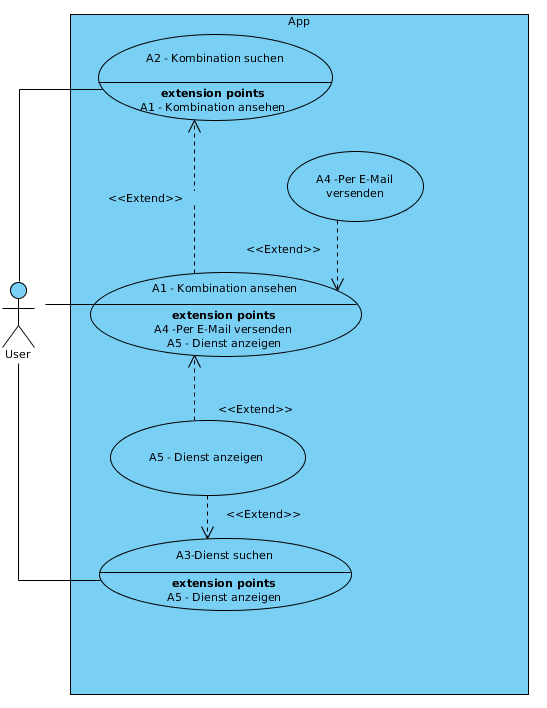
\includegraphics[keepaspectratio,width=11cm]{img/app}
	\caption{Anwendungsfalldiagramm - App}
	\label{fig:anwendungsfalldiagramm-app}
\end{figure}

\newpage

\begin{figure}[h]
	\centering
	\begin{tabularx}{\textwidth}{ X | X }
		\textbf{Anwendungsfall ID} & A4 \\ \hline
		\textbf{Anwendungsfallname} & Per E-Mail versenden \\ \hline
		\textbf{Initiierender Akteur} & Benutzer \\ \hline
		\textbf{Weitere Akteure} & -  \\ \hline
		\textbf{Kurzbeschreibung} & Der Benutzer hat bei der Ansicht einer Kombination die Möglichkeit, diese per E-Mail zu versenden. Dabei wird eine PDF generiert und das Standard E-Mail Programm wird geöffnet.  \\ \hline
		\textbf{Vorbedingungen} & Man hat eine nicht leere Kombination geöffnet.  \\ \hline
		\textbf{Nachbedingungen} & Die Standard E-Mail App wurde geöffnet und enthält das PDF im Anhang.  \\ \hline
		\textbf{Ablauf} &
			\begin{enumerate}
				\item Der Benutzer klickt auf den E-Mail senden Knopf.
        \item Eine PDF Datei wird generiert.
				\item Das Standard E-Mail Programm wird mit der PDF Datei im Anhang geöffnet.
			\end{enumerate} \\ \hline
		\textbf{Alternative} &
			- \\ \hline
		\textbf{Ausnahme} &
			- \\ \hline
		\textbf{Benutzte Anwendungsfälle} & - \\ \hline
	\end{tabularx}
	\caption{Anwendungsfall A4}
	\label{fig:anwendungsfall-app-tabelle-xx-1}
\end{figure}

\newpage


%%%%%%%%%%%%%%%
%% Anwendungsfall 2 %%
%%%%%%%%%%%%%%%

\section{Anwendungsfalldiagramm - Server}

\begin{figure}[h]
	\centering
	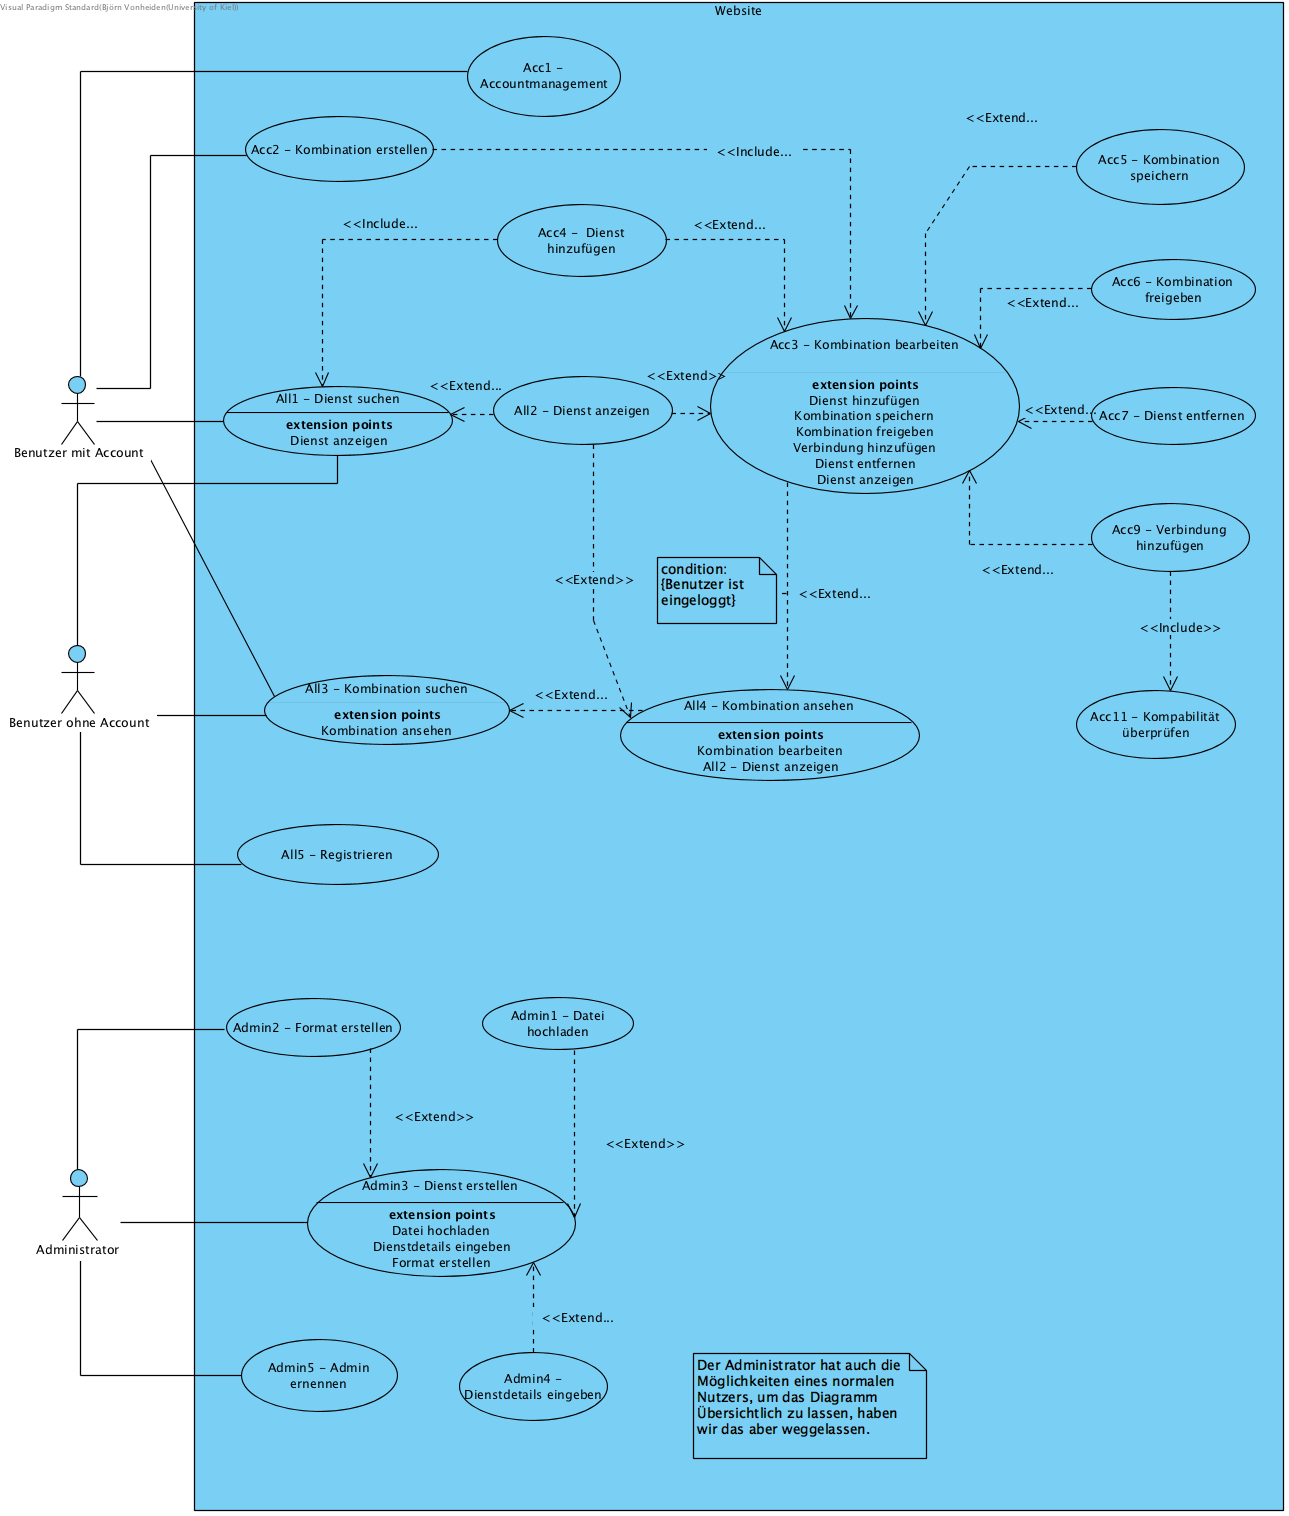
\includegraphics[width=\textwidth,height=15.5cm,keepaspectratio]{img/website}
	\caption{Anwendungsfalldiagramm - Server}
	\label{fig:anwendungsfalldiagramm-server}
\end{figure}

\newpage

\begin{figure}[h]
	\centering
	\begin{tabularx}{\textwidth}{ X | X }
		\textbf{Anwendungsfall ID} & Acc2 \\ \hline
		\textbf{Anwendungsfallname} & Kombination erstellen \\ \hline
		\textbf{Initiierender Akteur} & Benutzer mit Account / Administrator \\ \hline
		\textbf{Weitere Akteure} & -  \\ \hline
		\textbf{Kurzbeschreibung} & Erstellung einer Kombination um Kompatibilität der Dienste zu überprüfen.  \\ \hline
		\textbf{Vorbedingungen} & Der Benutzer besitzt einen Account und ist eingeloggt.  \\ \hline
		\textbf{Nachbedingungen} & -  \\ \hline
		\textbf{Ablauf} &
		\begin{enumerate}
			\item Der Nutzer möchte eine Kombination erstellen und bekommt eine leere Kombination angezeigt.
			\item {[Use-Case: Kombination bearbeiten]}
		\end{enumerate} \\ \hline
		\textbf{Alternative} &
			- \\ \hline
		\textbf{Ausnahme} &
      -  \\ \hline
		\textbf{Benutzte Anwendungsfälle} &
      \begin{itemize}
        \item Kombination bearbeiten
      \end{itemize} \\ \hline
	\end{tabularx}
	\caption{Anwendungsfall Acc2}
	\label{fig:anwendungsfall-server-tabelle-xx-1}
\end{figure}

\begin{figure}[h]
	\centering
	\begin{tabularx}{\textwidth}{ X | X }
		\textbf{Anwendungsfall ID} & Admin3 \\ \hline
		\textbf{Anwendungsfallname} & Dienst erstellen \\ \hline
		\textbf{Initiierender Akteur} & Administrator\\ \hline
		\textbf{Weitere Akteure} & -  \\ \hline
		\textbf{Kurzbeschreibung} & Ein Administrator kann entweder über eine Webschnittstelle oder über eine Datei einen neuen Dienst erstellen.  \\ \hline
		\textbf{Vorbedingungen} & Der Nutzer ist eingeloggt und besitzt Administratorrechte.  \\ \hline
		\textbf{Nachbedingungen} & Der Dienst wurde erstellt und ist jetzt von allen Nutzern sichtbar.  \\ \hline
		\textbf{Ablauf} &
		\begin{enumerate}
			\item Administrator wählt Webschnittstelle.
      \item {[Use-Case: Format erstellen]}
			\item {[Use-Case: Dienstdetails eingeben]}
			\item Der Administrator speichert den Dienst.
		\end{enumerate} \\ \hline
		\textbf{Alternative} &
    \begin{enumerate}
			\item Administrator wählt Dateischnittstelle.
			\item {[Use-Case: Datei hochladen]}
			\item Der Administrator speichert die hinzugefügten Dienste.
		\end{enumerate} \\ \hline
		\textbf{Ausnahme} &
    \begin{enumerate}
			\item Administrator wählt Webschnittstelle.
			\item {[Use-Case: Dienstdetails eingeben]}
			\item Der Administrator speichert den Dienst.
      \item Der Administrator bekommt eine Fehlermeldung, da Dienst schon vorhanden.
		\end{enumerate} \\ \hline
    \textbf{Ausnahme 2} &
		\begin{enumerate}
			\item Der Administrator wählt Datei hochladen.
			\item {[Use-Case: Datei hochladen]}
			\item Datei kann nicht gelesen werden, es gibt eine Fehlermeldung.
			\item Der Administrator kann eine neue Datei auswählen oder abbrechen.
		\end{enumerate}  \\ \hline
		\textbf{Benutzte Anwendungsfälle} &
    \begin{itemize}
			\item Datei hochladen
			\item Dienstdetails eingeben
      \item Format erstellen
		\end{itemize} \\ \hline
	\end{tabularx}
	\caption{Anwendungsfall Admin3}
	\label{fig:anwendungsfall-server-tabelle-xx-1}
\end{figure}
\begin{figure}[h]
	\centering
	\begin{tabularx}{\textwidth}{ X | X }
		\textbf{Anwendungsfall ID} & Acc3 \\ \hline
		\textbf{Anwendungsfallname} & Kombination bearbeiten \\ \hline
		\textbf{Initiierender Akteur} & Benutzer mit Account\\ \hline
		\textbf{Weitere Akteure} & -  \\ \hline
		\textbf{Kurzbeschreibung} & Ein Nutzer kann eine Kombination erstellen und bearbeiten.  \\ \hline
		\textbf{Vorbedingungen} & Der Nutzer ist eingeloggt und es gibt Kombination.  \\ \hline
		\textbf{Nachbedingungen} & -  \\ \hline
		\textbf{Ablauf} &
		\begin{enumerate}
      \item {[Use-Case: Dienst hinzufügen]} (ggf. mehrmals)
			\item {[Use-Case: Dienst entfernen]} (ggf. mehrmals)
			\item {[Use-Case: Verbindung hinzufügen]}
			\item {[Use-Case: Kombination speichern]}
			\item {[Use-Case: Kombination freigeben]}
		\end{enumerate} \\ \hline
		\textbf{Alternative} &
		\begin{enumerate}
			\item {[Use-Case: Dienst entfernen]}
			\item {[Use-Case: Kombination speichern]}
		\end{enumerate}  \\ \hline
		\textbf{Ausnahme} &
		- \\ \hline
		\textbf{Benutzte Anwendungsfälle} &
    \begin{itemize}
			\item Dienst hinzufügen
			\item Dienst entfernen
      \item Verbindung hinzufügen
      \item Kombination speichern
      \item Kombination freigeben
		\end{itemize} \\ \hline
	\end{tabularx}
	\caption{Anwendungsfall Acc3}
	\label{fig:anwendungsfall-server-tabelle-xx-1}
\end{figure}


	\chapter{Testfälle}\label{chp:testfaelle}
	\section{Testfälle Webseite}
\begin{figure}[!h]
	\begin{center}
		\begin{tabularx}{\textwidth}{ p{.05\textwidth} | p{.1\textwidth} | p{.35\textwidth} | X }
			\textbf{Nr.} & \textbf{ID} & \textbf{Szenario} & \textbf{Erwartetes Verhalten} \\ \hline
			1 & Acc1 &User ändert Passwort & Passwort wird geändert.\\ \hline
			2 & Acc1 &User ändert Organisation &Organisation wird geändert.\\ \hline
			3 & Acc3-Acc9 &Leere Kombination erstellen &Leere Kombination wird angezeigt.\\ \hline
			4 & Acc3-Acc4-Acc9 &5 Dienste hinzufügen verbinden  &Kombination wird errechnet und dargestellt. \\ \hline
			5 & Acc3-Acc4 &Dienste hinzufügen, nicht verbinden &Dienste werden angezeigt.\\ \hline
			6 & Acc2-Acc3-Acc5 &Kombination erstellen,  speichern &Kombination wird mit Namen gespeichert.\\ \hline
			7 & All4 &Kombination anzeigen &Gespeicherte Kombination wird angezeigt. \\ \hline
			8 & All4-Acc6 &Kombination für User X freigeben &User X hat zugriff auf Kombination.\\ \hline
			9 & All1 &User sucht Dienst &Alle passenden Dienste werden angezeigt.\\ \hline
			10 & Admin3-Admin4 &Admininistrator erstellt Dienst mit manueller Eingabe &Dienst wird mit eingegebenen Daten erstellt.\\ \hline
      11 & Admin3-Admin4 &Admininistrator erstellt Dienst mit manueller Eingabe und Dienst existiert schon &Dienst wird nicht erstellt.\\ \hline
			12 & Admin1-Admin3 &Admininistrator erstellt Dienst durch einlesen von Datei &Dienst mit Daten aus Datei wird erstellt. \\ \hline
			13 & Admin5 &Admininistrator ernennt User X zu Admininistrator &User X hat Administratorechte.\\ \hline
			\end{tabularx}
	\end{center}
	\caption{wichtige Testfälle Webseite}
	\label{fig:testfaelle-tabelle}
\end{figure}
\newpage
\section{Testfälle App}
\begin{figure}[!h]
	\begin{center}
		\begin{tabularx}{\textwidth}{ p{.05\textwidth} | p{.1\textwidth} | p{.35\textwidth} | X }
			\textbf{Nr.} & \textbf{ID} & \textbf{Szenario} & \textbf{Erwartetes Verhalten} \\ \hline
			1 & A1 & Kombination anklicken und ansehen & Kombination wird angezeigt.\\ \hline
			2 & A2-A1  & Kombination suchen und ansehen & Gesuchte Kombination wird angezeigt.\\ \hline
			3 & A1-A4-A6 & Kombination per E-Mail senden & PDF wird generiert und Standard E-Mail-Programm wird geöffnet.\\ \hline
			4 & A3 & Dienst suchen & Liste an Diensten wird angezeigt.\\ \hline
			5 & A3-A5 & Dienst suchen und anzeigen & Gesuchter Dienst wird angezeigt.\\ \hline
			6 &  A1-A5 & Dienst einer Kombination anzeigen & Dienst wird angezeigt.
			\end{tabularx}
	\end{center}
	\caption{wichtige Testfälle App}
	\label{fig:testfaelle-tabelle}
\end{figure}


	\chapter{Produktdaten}\label{chp:produktdaten}
	In diesem Kapitel wird festgehalten, welche Daten mit welchen Attributen die Software verarbeitet bzw. speichert.
\begin{enumerate}
	\item \textit{Benutzerinformationen:}
	Nachname, Vorname, Titel, Organisation, E-Mail-Adresse, Passwort und Rolle werden zum Benutzer gespeichert.
	\item \textit{Dienst:} Name, Organisation, Version, Veröffentlichungsdatum, Tags, FormatIn/Out, Logo und ID werden zu
	jedem Dienst gespeichert.
	\item \textit{Format:} Zu den Formaten wird der Name, die Version und der Kompabilitätsgrad gespeichert.
	\item \textit{Kombination:} Jede Kombination bekommt eine ID, einen Namen, eine Liste von den kombinierten Diensten mit deren IDs, der jeweiligen Position im Bild und der Verbindungen der kombinierten Dienste.
	Außerdem wird eine Liste gespeichert in der die IDs der Nutzer stehen, für welche die Kombination freigegeben ist.
\end{enumerate}


	\chapter{Benutzeroberfläche}\label{chp:benutzeroberflaeche}
	\section{App}
Die App soll den Features entsprechend schlicht gehalten werden.
So können wir die Nutzung der App intuitiv, einfach und schnell gestalten.
Der Benutzer soll sofort wissen wie er die App nutzen kann ohne eine entsprechende Einweisung.

\begin{figure}[ht]
	\centering
	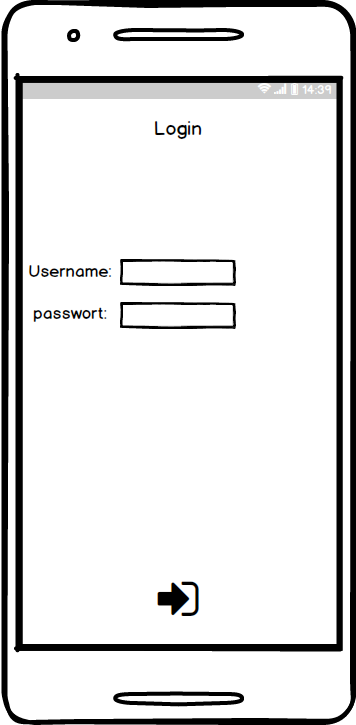
\includegraphics[keepaspectratio,width=5cm]{img/Login}
	\caption{Schlichte Login Seite}
	\label{fig:App1}
\end{figure}

\begin{figure}[ht]
	\centering
	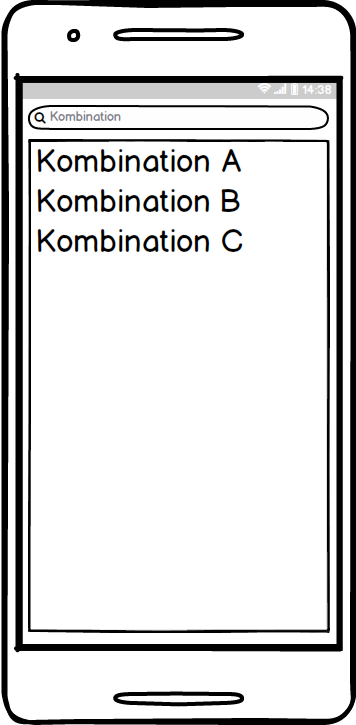
\includegraphics[keepaspectratio,width=8cm]{img/Kombination_suchen}
	\caption{Suchen nach gespeichterten Kombinationen}
	%\label{fig:mock-pw}
\end{figure}

\begin{figure}[ht]
	\centering
	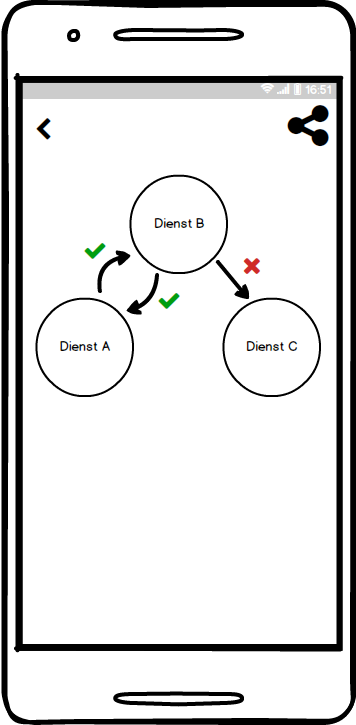
\includegraphics[keepaspectratio,width=8cm]{img/Kombination_anzeigen_Verbunden}
	\caption{Anzeigen einer Kombination}
	%\label{fig:mock-pw}
\end{figure}

\begin{figure}[ht]
	\centering
	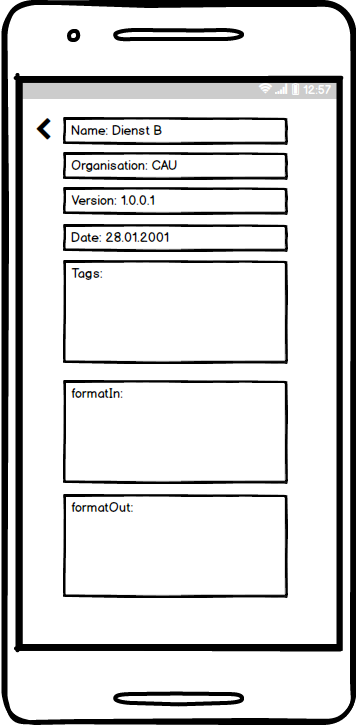
\includegraphics[keepaspectratio,width=8cm]{img/Dienst_anzeigen_Dienst_B}
	\caption{Darstellung eines einzelnen Dienstes}
	%\label{fig:mock-start}
\end{figure}

\begin{figure}[ht]
	\centering
	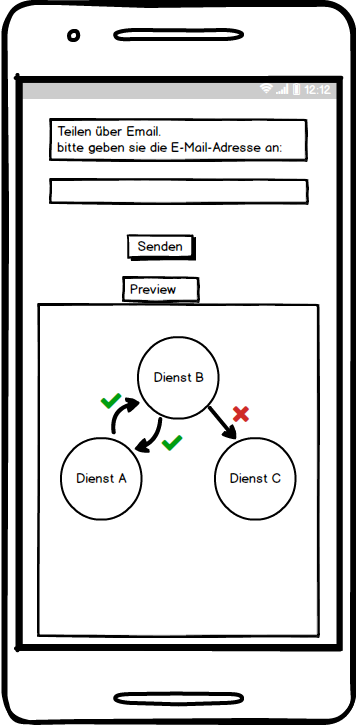
\includegraphics[keepaspectratio,width=8cm]{img/Kombination_teilen}
	\caption{Mögliches Teilen per Email einer Kombination}
	%\label{fig:mock-pw}
\end{figure}

\section{Webseite}
Auf der Webseite können von jedem Benutzer Dienstkombinationen angelegt und bearbeitet werden.
Diese Kombinationen werden gespeichert und ggf. für weitere Benutzer freigegeben.
Das Verknüpfen von jeweils zwei Diensten geschieht mittels Drag \& Drop.
Sollten miteinander verknüpfte Dienste nicht kompatibel zueinander sein, kann die Software alternative Vorschläge anzeigen, um diese Inkompatibilität aufzulösen.
Zusätzlich dürfen Administratoren Dienste und Eingabe- bzw. Ausgabeformate verwalten.
Eine einfache Benutzerverwaltung soll ebenfalls eingebaut werden, die es Administratoren erlaubt,
Benutzern Administratorenrechte zu geben oder wieder zu entziehen.
Obwohl die Webseite deutlich komplexer sein wird als die App, soll auch hier der Fokus auf Benutzerfreundlichkeit und einer intuitiven Bedienung gesetzt werden. Auch ohne Einweisung soll es dem Benutzer schnell gelingen, beliebige Kombinationen von Diensten zu erstellen.

\begin{figure}[ht]
	\centering
	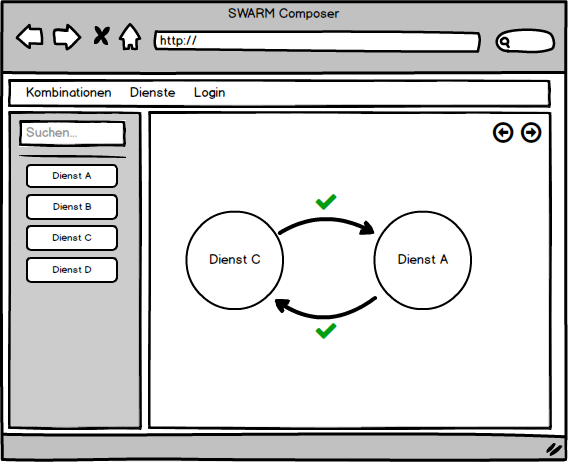
\includegraphics[keepaspectratio,width=11cm]{img/webfrontend/Kombinationen_Detail_Anonym.png}
	\caption{Darstellung einer Kombination ohne Account.}
	%\label{fig:mock-web-combination}
\end{figure}

\begin{figure}[ht]
	\centering
	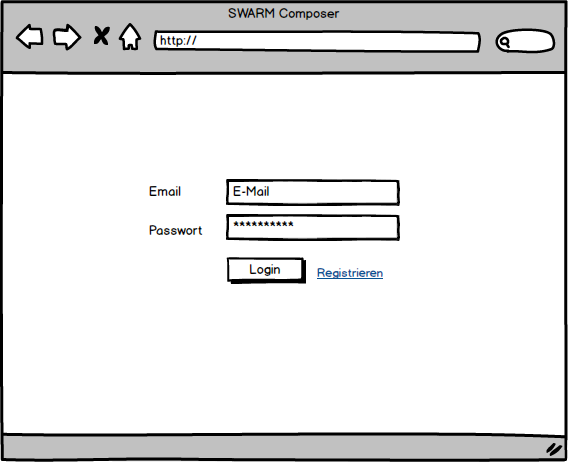
\includegraphics[keepaspectratio,width=11cm]{img/webfrontend/Login.png}
	\caption{Login}
	%\label{fig:mock-web-login}
\end{figure}

\begin{figure}[ht]
	\centering
	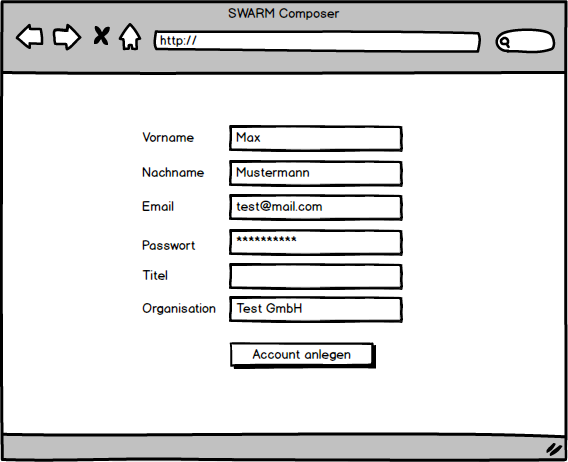
\includegraphics[keepaspectratio,width=11cm]{img/webfrontend/Registrieren.png}
	\caption{Neuen Account erstellen}
	%\label{fig:mock-web-register}
\end{figure}
\begin{figure}[ht]
	\centering
	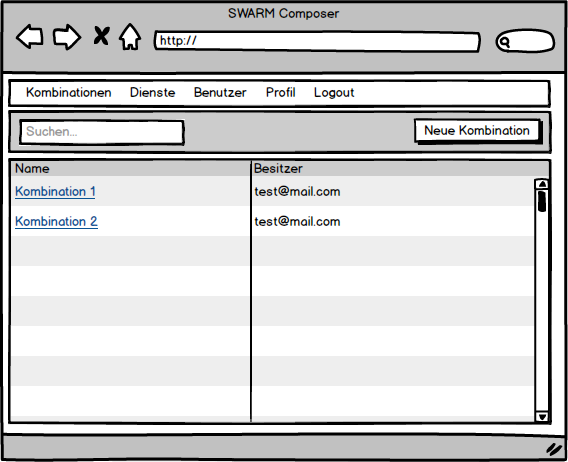
\includegraphics[keepaspectratio,width=11cm]{img/webfrontend/Kombinationen.png}
	\caption{Auflistung der Dienstkombinationen}
	%\label{fig:mock-web-combinations}
\end{figure}

\begin{figure}[ht]
	\centering
	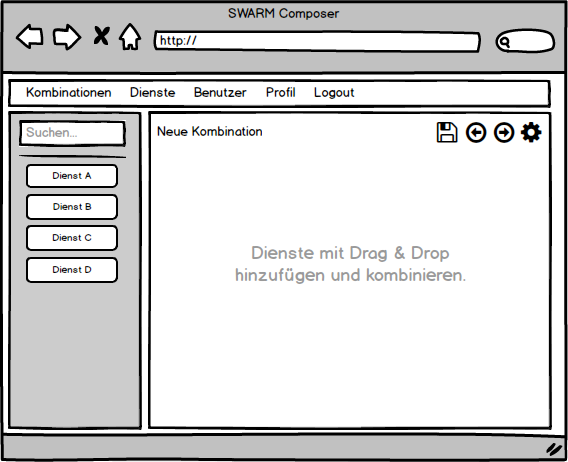
\includegraphics[keepaspectratio,width=11cm]{img/webfrontend/Kombinationen_Leer.png}
	\caption{Eine leere Kombination ohne Dienste}
	%\label{fig:mock-web-emptycombination}
\end{figure}

\begin{figure}[ht]
	\centering
	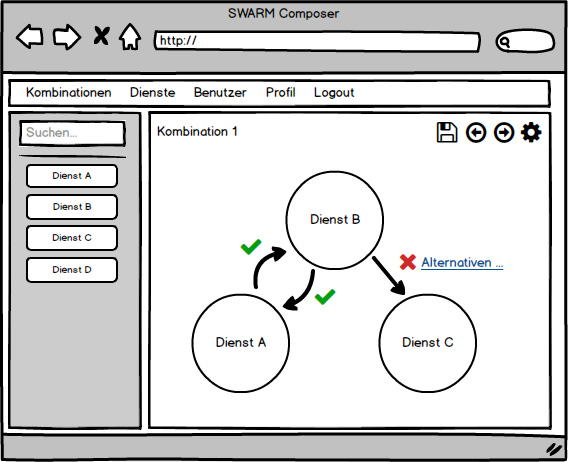
\includegraphics[keepaspectratio,width=11cm]{img/webfrontend/Kombinationen_Detail.png}
	\caption{Eine Kombination, die mehrere Dienste miteinander verknüpft. 'Dienst B' und 'Dienst C' sind inkombatibel}
	%\label{fig:mock-web-combination}
\end{figure}

\begin{figure}[ht]
	\centering
	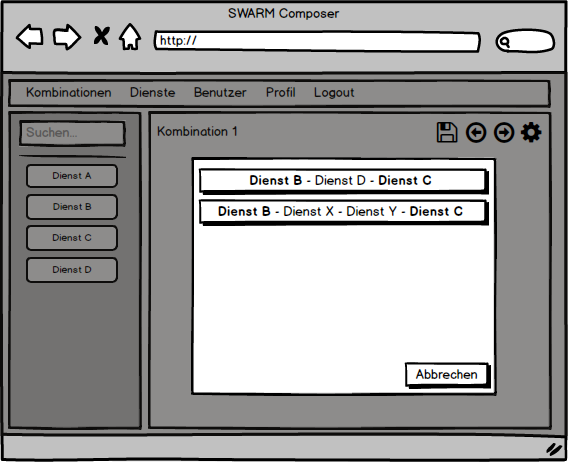
\includegraphics[keepaspectratio,width=11cm]{img/webfrontend/Kombinationen_Alternativen.png}
	\caption{Alternativen zu inkompatiblen Diensten}
	%\label{fig:mock-web-alternatives}
\end{figure}

\begin{figure}[ht]
	\centering
	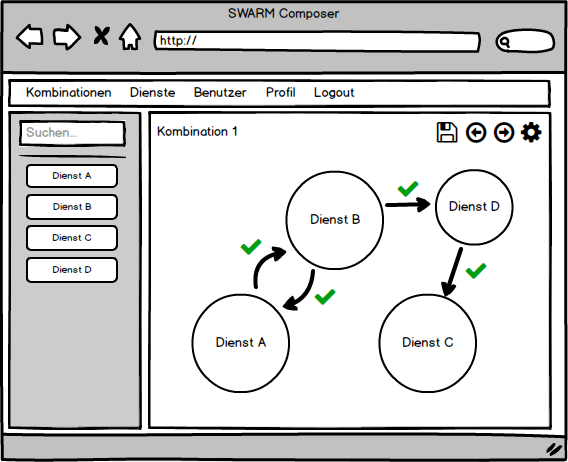
\includegraphics[keepaspectratio,width=11cm]{img/webfrontend/Kombinationen_Details_Neu.png}
	\caption{Alternative Dienste werden automatisch eingefügt}
	%\label{fig:mock-web-combinationalt}
\end{figure}

\begin{figure}[ht]
	\centering
	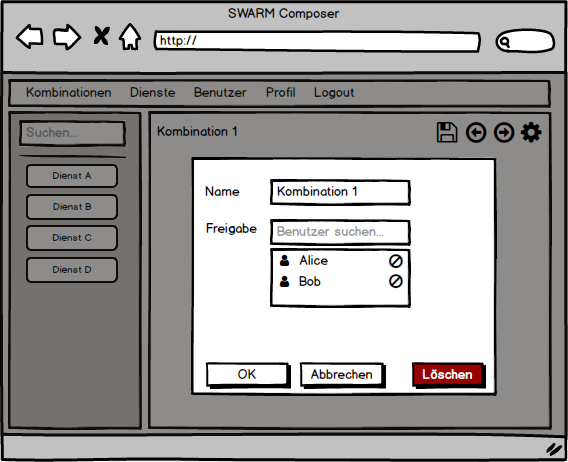
\includegraphics[keepaspectratio,width=11cm]{img/webfrontend/Kombinationen_Optionen.png}
	\caption{Details zu einer Kombination}
	%\label{fig:mock-web-combinationdialog}
\end{figure}

\begin{figure}[ht]
	\centering
	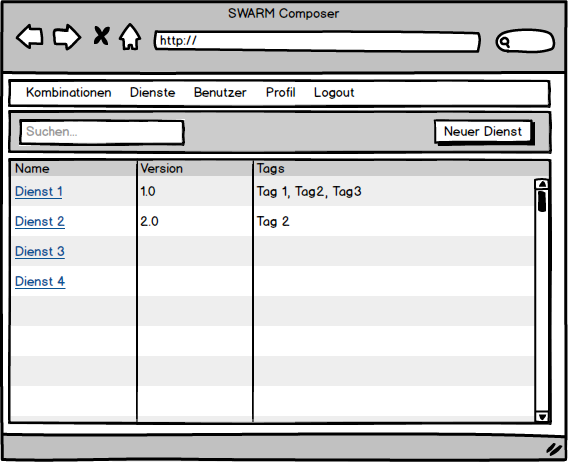
\includegraphics[keepaspectratio,width=11cm]{img/webfrontend/Dienste.png}
	\caption{Auflistung der Dienste}
	%\label{fig:mock-web-services}
\end{figure}

\begin{figure}[ht]
	\centering
	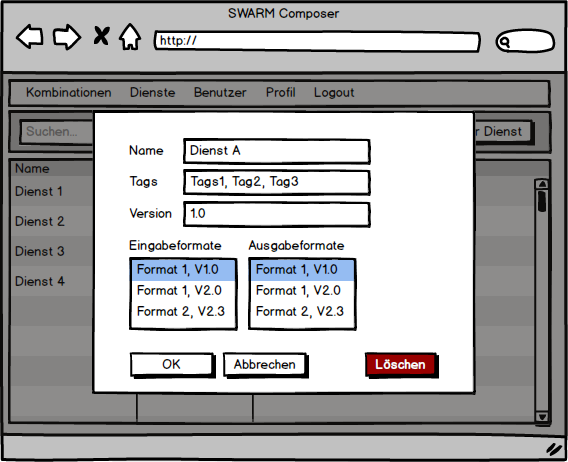
\includegraphics[keepaspectratio,width=11cm]{img/webfrontend/Dienste_Detail.png}
	\caption{Details zu einem Dienst}
	%\label{fig:mock-web-servicedetail}
\end{figure}

\begin{figure}[ht]
	\centering
	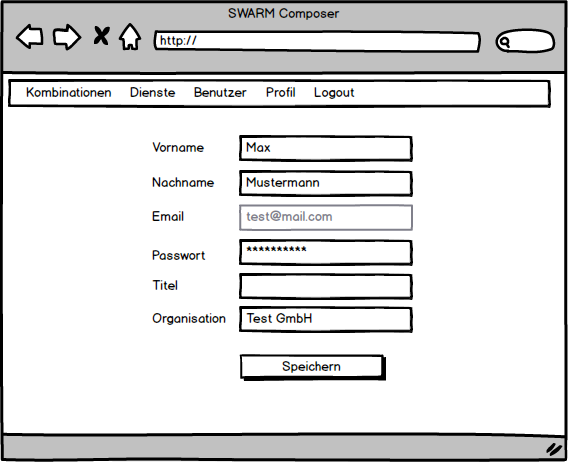
\includegraphics[keepaspectratio,width=11cm]{img/webfrontend/Profil.png}
	\caption{Benutzer können ihre gespeicherten Daten einsehen und ändern.}
	%\label{fig:mock-web-formats}
\end{figure}

\begin{figure}[ht]
	\centering
	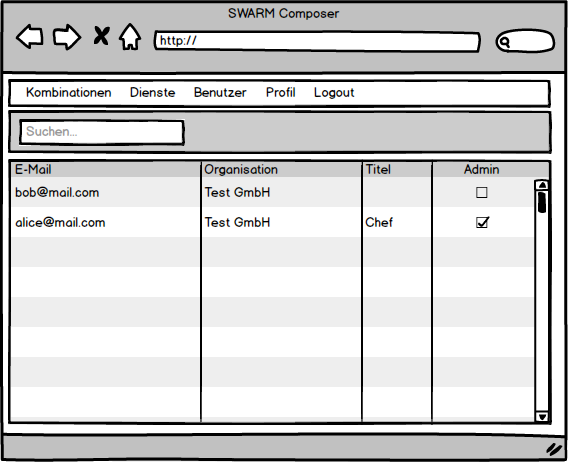
\includegraphics[keepaspectratio,width=11cm]{img/webfrontend/Benutzer.png}
	\caption{Auflistung der Benutzer.}
	%\label{fig:mock-web-users}
\end{figure}


	\chapter{Qualitätsanforderung}\label{chp:qualitaetsanforderung}
	Bei der Software ist es besonders wichtig, dass die Zuverlässigkeit gewährleistet ist.
Kunden müssen sich darauf verlassen können, dass die Software richtige Ergebnisse liefert, da Sie sonst den Service nicht nutzen.
Des Weiteren  ist ein hoher Stellenwert der Benutzerfreundlichkeit einzuräumen.
Besonders mit Augenmerk auf den erwarteten Kundenstamm muss darauf geachtet werden, dass sowohl die App als auch die Webseite leicht zu bedienen sind und gut aussehen.
Als dritter, sehr wichtiger Aspekt ist die Erweiterbarkeit zu nennen.
Bei ständig neu entwickelten Diensten und Formaten ist es dringend notwendig, dass die Software schnell und einfach um diese erweitert werden kann.
Immernoch wichtig, aber mit einer geringeren Priorität, werden Robustheit, Wartbarkeit, Effizenz und Sicherheit eingeschätzt.
Ein gewisses Maß an Robustheit ist wichtig, jedoch sind einzelne Abstürzt ohne Datenverlust ohne große Konsequenzen.
Ähnlich ist es bei der Wartbarkeit.
Da es kein kritisches System ist, können Fehler mittelfristig bestehen ohne die Lauffähigkeit zu gefährden.
Da mit Datenbanken gearbeitet wird, die schnell groß werden, muss besonders darauf geachtet werden, dass die Lookup-Zeiten (Zugriffszeit auf die Daten) gering gehalten werden, um so bei komplexen Kombinationen ein Ergebnis zügig erzeugen zu können.
Die Kommunikation zwischen App, Webseite und Server muss geschützt werden.
Da jedoch keine hochkritischen Daten geteilt werden, reicht ein normaler Fokus auf die Sicherheit.
Für die Software weniger wichtig ist Anpassbarkeit und Kompatibilität anzusehen.
Durch eine einfache Benutzeroberfläche mit voller Funktionalität besteht eine geringe Notwendigkeit die Oberfläche anzupassen.
Da der Umgebungsbereich der Software klar definiert ist, muss hier nicht groß darauf geachtet werden, eine möglichst offene API zu entwickeln.


\begin{table}[h]
	\centering
	\begin{tabularx}{\textwidth}{l c c c c}
		\rowcolor[HTML]{C0C0C0}
		& \textbf{sehr wichtig} & \textbf{wichtig} & \textbf{weniger wichtig} & \textbf{unwichtig} \\
		Robustheit &  & x  &  &  \\
		\rowcolor[HTML]{E7E7E7}
		Zuverlässigkeit & x &  &  &  \\
		Wartbarkeit &  & x &  &  \\
		\rowcolor[HTML]{E7E7E7}
		Erweiterbarkeit & x &  &  &  \\
		Benutzerfreundlichkeit & x &  &  &  \\
		\rowcolor[HTML]{E7E7E7}
		Effizienz &  & x &  &  \\
		Anpassbarkeit &  &  & x &  \\
		\rowcolor[HTML]{E7E7E7}
		Kompatibilität &  & & x  &  \\
		Sicherheit &  &  x & &
	\end{tabularx}
	\caption{Qualitätsanforderungen}
	\label{tabelle:qualitaetsanforderungen}
\end{table}


	\chapter{Glossar}\label{chp:glossar}
	\begin{table}[h]
	\centering
	\begin{tabularx}{\textwidth}{X X}
		\rowcolor[HTML]{C0C0C0}
		\textbf{Abkürzung} & \textbf{Beschreibung} \\
		API & Application Programming Interface \\
		\rowcolor[HTML]{E7E7E7}
		CPU & Cental Processing Unit \\
		JSON & JavaScript Object Notation \\
		\rowcolor[HTML]{E7E7E7}
		RAM & Random-Access Memory \\
		REST & Representational State Transfer \\
		\rowcolor[HTML]{E7E7E7}
		Lookup-Zeit & Zugriffszeit auf die Daten \\
	\end{tabularx}
	\caption{Glossar}
	\label{table:glossar}
\end{table}


	\bibliography{references}
	\pagenumbering{gobble} % Nummerierung deaktivieren

\end{document}
